\documentclass{beamer}
\usetheme{Madrid}
\usecolortheme{default}

% ---------- math + figures ----------
\usepackage{amsmath, amssymb, bm}
\usepackage{graphicx}
\usepackage{hyperref}
\usepackage{tikz}
\usepackage{xcolor}
\usetikzlibrary{tikzmark, calc, fit}
\usetikzlibrary{patterns} % needed for hatch patterns
\usepackage{listings}
\usepackage{mathtools}
\usepackage{pgfplots}
\usepackage{xcolor}  % usually already loaded by Beamer
% \definecolor{mycreamy}{RGB}{153,76,0}  % define your own color
% \setbeamercolor{structure}{fg=mycreamy}
% ---------- algo / theorem helpers ----------
\usepackage{algorithm}
\usepackage{algpseudocode}     % nice pseudocode
\usepackage[skins]{tcolorbox}  % shaded theorem blocks
\usepackage{mdframed}

% ---------- title + metadata ----------
\title[Thompson Sampling for BCO]{Thompson Sampling for Bandit Convex Optimisation}
\author{Alireza Bakhtiari$^1$ \and Tor Lattimore$^2$ \and Csaba Szepesvári$^{1,2}$}
\institute{University of Alberta$^1$ \quad \& \quad Google DeepMind$^2$}
\date{COLT 2025}

\setbeamertemplate{navigation symbols}{}
\setbeamertemplate{footline}{
  \leavevmode%
  \hfill%
  \usebeamerfont{page number in head/foot}%
  \usebeamercolor[fg]{page number in head/foot}%
  \insertframenumber{} / \inserttotalframenumber\hspace{1em}\vskip2pt%
}

%-------- plot params ----------
\newcommand\epsval{0.2}        % ε ∈ [0,1/2]
\def\thetazero{1}              % θ_x component
\def\thetaone{0}               % θ_y component
\pgfmathsetmacro\radtest{1+2*\epsval}     % threshold 1+2ε
\pgfmathsetmacro\sqrtt{sqrt(\radtest)}    % √(1+2ε)

%---------- shorthand ----------
\newcommand{\ip}[1]{\left \langle #1 \right \rangle}
\newcommand{\lip}{\operatorname{Lip}}
\newcommand{\ball}{\mathbb{B}}
\newcommand{\sphere}{\mathbb{S}}
\newcommand{\norm}[1]{\left \Vert  #1 \right \Vert}
\newcommand{\Reg}{\operatorname{Reg}}
\newcommand{\BReg}{\operatorname{BReg}}
\newcommand{\pair}{\operatorname{\textsc{pair}}}
\newcommand{\dis}{\operatorname{\textsc{dis}}}
\newcommand{\diam}{\operatorname{diam}}
\newcommand{\conv}{\operatorname{conv}}
\newcommand{\argmin}{\operatornamewithlimits{argmin}}
\newcommand{\argmax}{\operatornamewithlimits{argmax}}
\newcommand{\E}{\mathbb{E}}
\newcommand{\PP}{\mathbb{P}}
\newcommand{\R}{\mathbb{R}}
\newcommand{\cK}{\mathcal{K}}
\newcommand{\cF}{\mathcal{F}}
\newcommand{\cA}{\mathcal{A}}
\newcommand{\cP}{\mathcal{P}}
\newcommand{\cI}{\mathcal{I}}
\newcommand{\ts}{{\textsc{ts}}}
\newcommand{\pr}{\text{\tiny\texttt{r}}}
\newcommand{\pb}{\text{\tiny\texttt{b}}}
\newcommand{\pl}{\text{\tiny\texttt{l}}}
\renewcommand{\pm}{\text{\tiny\texttt{m}}}
\newcommand{\IR}{\operatorname{\textsc{ir}}}
\newcommand{\ceil}[1]{\left\lceil #1 \right\rceil}
\newcommand{\floor}[1]{\left\lfloor #1 \right\rfloor}


%%%%%%%%%%%%%%%%%%%%%%%%%%%%%%%%%%%%%%%%%%%%%%%%%%%%
%%%%%%%%%%%%%%%%%%%%%%%%%%%%%%%%%%%%%%%%%%%%%%%%%%%%
%%%%%%%%%%%%%%%%%%%%%%%%%%%%%%%%%%%%%%%%%%%%%%%%%%%%
%%%%%%%%%%%%%%%%%%%%%%%%%%%%%%%%%%%%%%%%%%%%%%%%%%%%
%%%%%%%%%%%%%%%%%%%%%%%%%%%%%%%%%%%%%%%%%%%%%%%%%%%%
%%%%%%%%%%%%%%%%%%%%%%%%%%%%%%%%%%%%%%%%%%%%%%%%%%%%
\begin{document}

%%%%%%%%%%%%%%%%%%%%%%%%%%%%%%%%%%%%%%%%%%%%%%%%%%%%
\begin{frame}
    \titlepage
\end{frame}

%%%%%%%%%%%%%%%%%%%%%%%%%%%%%%%%%%%%%%%%%%%%%%%%%%%%
\begin{frame}{Paper in One Slide}
    \begin{itemize}
        \item \alert{Goal}: Understand how \textbf{Thompson Sampling (TS)} behaves in \textbf{bandit convex optimization (BCO)}.
        \item \textbf{Positive}:
              \begin{itemize}
                  \item $\BReg_n(\ts) = \widetilde{O}(\sqrt{n})$ in \emph{1-D} convex bandits.
                  \item $\BReg_n(\ts) = \widetilde{O}\!\bigl(d^{2.5}\sqrt{n}\bigr)$ for \emph{d-D monotone convex ridge} losses.
              \end{itemize}
        \item \textbf{Negative}:
              \begin{itemize}
                  \item TS can suffer \(\Omega(\exp(d))\) regret for general d-D convex losses.
                  \item Classical info-ratio tricks \(\Rightarrow\) no better than \(\widetilde{O}(d^{1.5}\sqrt{n})\) for general stochastic \& adversarial BCO.
              \end{itemize}
              % \item \textbf{Take-away}: TS is great in 1-D / structured convex settings, but not in full \(d\)-D.
    \end{itemize}
\end{frame}

%%%%%%%%%%%%%%%%%%%%%%%%%%%%%%%%%%%%%%%%%%%%%%%%%%%%
\begin{frame}{Problem Setup}
    \begin{itemize}
        \item Convex action set \( \cK \subset \mathbb{R}^d \).
        \item $\cF$ be a set of convex functions from $\cK$ to $[0,1]$.
        \item $\xi$ is a known prior on $\cF$.
        \item<2-> At round \(t\):
              \begin{enumerate}
                  \item Learner plays \(X_t \in \cK\).
                  \item Observes scalar loss \( Y_t \in \{0,1\}\).\footnote{The Bernoulli noise assumption is just for convenience.}
              \end{enumerate}
        \item<3-> $\E\left[Y_t|X_1, Y_1, \cdots, X_t, f\right] = f(X_t)$, where $f \in \cF$ is convex.
        \item<4-> $\cA$ (learner) is a mapping from histories $\&$ prior to $\cK$.
        \item<5-> \textbf{Bayesian Regret}
              \[
                  \BReg_n(\cA, \xi) =
                  \E\left[
                      \sup_{x \in \cK}
                      \sum_{t=1}^n (f(X_t) - f(x))
                      \right]\,,
              \]
              where $f\sim \xi$.
    \end{itemize}
\end{frame}

%%%%%%%%%%%%%%%%%%%%%%%%%%%%%%%%%%%%%%%%%%%%%%%%%%%%
\begin{frame}{Thompson Sampling for BCO}
    \begin{algorithm}[H]
        \caption{Thompson Sampling}
        \begin{algorithmic}[1]
            \State Prior \( \xi \) over convex losses.
            \For{\(t = 1,\dots, n\)}
            \State Sample \(f_t \sim \PP(f=\cdot|X_1, Y_1, \cdots, X_{t-1}, Y_{t-1})\)
            \State Play \( X_t \in \arg\min_{x\in\cK} f_t(x) \) and observe $Y_t$
            \EndFor
        \end{algorithmic}
    \end{algorithm}
    \begin{itemize}
        \item Our analysis studies how
              \[
                  \BReg^{\ts}(\cF) = \sup_{\xi \in \cP(\cF)} \BReg_n(\ts, \xi)\,,
              \]
              behaves for various natural classes of convex functions $\cF$.
    \end{itemize}
\end{frame}

%%%%%%%%%%%%%%%%%%%%%%%%%%%%%%%%%%%%%%%%%%%%%%%%%%%%
\begin{frame}{Upper bounds - main results}
    \begin{itemize}
        \item Positive results for two sets of functions $f:\cK \to [0,1]$:\vspace{1em}
              \begin{enumerate}
                  \large
                  \setlength{\itemsep}{1em} % Adjust the spacing (1em is an example)
                  \item[$\cF_{\pb\pl}$]: $\cK \subset \R$ and $f$ is a 1-Lip and bounded convex function,
                  \item[$\cF_{\pb\pl\pr\pm}$] : $\cK \subset \R^d$ and $f(x) = \ell(\langle x, \theta\rangle)$ for some $\theta\in\R^d$ and a convex 1-Lip bounded \emph{monotone} $\ell: \R \to \R$.
              \end{enumerate}
    \end{itemize}
    \begin{tcolorbox}[title=Upper bounds -- 1-D convex functions,colback=blue!5!white,colframe=blue!50!black]
        TS achieves
        \[
            \BReg^{\ts}(\cF_{\pb\pl})\;=\; \widetilde{O}\!\bigl(\sqrt{n}\bigr)\,,
        \]
        And
        \[
            \BReg^{\ts}(\cF_{\pb\pl\pr\pm})\;=\; \widetilde{O}\!\bigl(d^{2.5}\sqrt{n}\bigr)\,.
        \]
    \end{tcolorbox}
\end{frame}

%%%%%%%%%%%%%%%%%%%%%%%%%%%%%%%%%%%%%%%%%%%%%%%%%%%%

\begin{frame}{Upper bounds -- analysis}
    (Generalized) \textbf{Information Ratio (IR)}
    \vspace{0.5em}
    \small
    \begin{itemize}
        \item Let $x_g = \argmin_{x\in\cK} g(x)$. (analysis is really about $x_f$ and $f(x_f)$.)
        \item Let $(X,f)$ have law $\pi \otimes \xi,$ and $\bar{f} = \E[f]$.
        \item Define
              \begin{align*}
                  \Delta(\pi, \xi) = \E[\bar{f}(X) - f_\star]
                  \quad \text{and} \quad \cI(\pi, \xi) = \E[(f(X) - \bar{f}(X))^2]\,.
              \end{align*}
    \end{itemize}
    \begin{tcolorbox}[title=Generalized IR ,colback=green!5!white,colframe=green!50!black]
        Define generalized information ratio associated with $\ts$ as
        \[
            \IR(\cF) = \left\{(\alpha, \beta) \in \R_+^2 : \Delta(\pi_{\ts}, \xi) \leq \alpha + \sqrt{\beta \cI(\pi_{\ts}, \xi)}  \;,\forall \xi\right\} \,.
        \]
    \end{tcolorbox}
    \begin{itemize}
        \item $(0,\beta) \in \IR(\cF) \Rightarrow \Delta(\pi_{\ts}, \xi)^2/\cI(\pi_{\ts}, \xi) \leq \beta$.
    \end{itemize}
\end{frame}

%%%%%%%%%%%%%%%%%%%%%%%%%%%%%%%%%%%%%%%%%%%%%%%%%%%%

\begin{frame}{Upper bounds -- regret \&\ IR}
    \small
    \begin{tcolorbox}[title=Proposition 1 -- regret bound through IR,colback=blue!5!white,colframe=blue!50!black]
        Suppose that $\cF \in \{\cF_{\pb\pl}, \cF_{\pb\pl\pr\pm}\}$ and $(\alpha, \beta) \in \IR(\cF)$.
        Then, the regret of $\ts$ is at most
        \begin{align*}
            \BReg_n(\ts, \xi) \leq n \alpha + O\left(\sqrt{\beta n d \log(n \diam(\cK))}\right) \,.
        \end{align*}
    \end{tcolorbox}
    \only<2-2>{It remains to bound the IR of $\ts$.}
    \uncover<3->{
        \begin{tcolorbox}[title=Proposition 2 -- $\ts$-IR Decomposition,colback=blue!5!white,colframe=blue!50!black]
            If $\exists k, m \in \mathbb{N} $ such that for all $\tilde f \in \conv(\cF)$ there is $\cF = \cup_{i=1}^m \cF_i$
            for which
            \begin{align*}
                \sup_{f \in \cF_i} (\tilde f(x_f) - f(x_f)) \leq \alpha + \sqrt{\beta
                \underbrace{\inf_{f_1,\ldots,f_k \in \cF_i} \sum_{j\neq l \in [k]} (f_j(x_{f_l}) - \tilde f(x_{f_l}))^2}_{\dis(\cF_i, k)}
                } \,,
            \end{align*}
            for all $i$, then $(\alpha, k(k-1)m\beta) \in \IR(\cF)$.
        \end{tcolorbox}
        \only<4->{
            \begin{tikzpicture}[remember picture, overlay]
                \draw[red, ultra thick, rounded corners]
                ([yshift=2pt]$(current page.center)+(-4.85,-1.5)$)
                rectangle
                ([yshift=-2pt]$(current page.center)+(-1.85,-2.5)$);
                \node[anchor=north, red] at
                ([yshift=2pt]$(current page.center)+(-3.35,-2.6)$)
                {worst case \emph{average} regret within $\cF_i$};
            \end{tikzpicture}
        }
        \only<5->{
            \begin{tikzpicture}[remember picture, overlay]
                \draw[red, ultra thick, rounded corners]
                ([yshift=2pt]$(current page.center)+(-0.22,-1.5)$)
                rectangle
                ([yshift=-2pt]$(current page.center)+(4.65,-3.1)$);
                \node[anchor=north, red] at
                ([yshift=2pt]$(current page.center)+(2,-3.2)$)
                {$\ts$ minimum inf. gain (discrepancy)};
            \end{tikzpicture}
        }
    }
\end{frame}

%%%%%%%%%%%%%%%%%%%%%%%%%%%%%%%%%%%%%%%%%%%%%%%%%%%%

\begin{frame}{Upper bounds -- IR bound in 1-D}
    \small
    \begin{tcolorbox}[title=Theorem 3 -- IR bound for 1-D,colback=blue!5!white,colframe=blue!50!black]
        Suppose that $d = 1$ and $\alpha \in (0,1)$. Then $(\alpha, 10^4 \ceil{\log(1/\alpha)}) \in \IR(\cF_{\pb\pl})$.
    \end{tcolorbox}
    \textbf{Proof sketch:}
    \begin{itemize}
        \item Use the decomposition lemma $\Rightarrow$ partition  based on $x_f$ and $f(x_f)$.
        \item Analyze functions with similar gaps (average regret) in $\cF_i$:
              \begin{enumerate}
                  \leftskip=4em % Add right padding of 2em
                  \item[Similar gaps:] $\bar{f}(x_f) - f(x_f) \in [\epsilon, 2\epsilon]$,
                  \item[$\bar{f}$ monotone:] $x_{\bar{f}} \leq x_f \Rightarrow $ $\bar{f}$ (begin 1-D is crucial here).
              \end{enumerate}
        \item Prove that $\dis(\cF_i, k) \geq c^2\epsilon_i^2$
              \[
                  \inf_{f_1,\ldots,f_k \in \cF_i} \sum_{j\neq l \in [k]} (f_j(x_{f_l}) - \tilde f(x_{f_l}))^2 \geq c^2\epsilon_i^2\,.
              \]
    \end{itemize}
\end{frame}

\begin{frame}{Upper bounds -- IR bound in 1-D}
    \small
    \textbf{Proof sketch:}(proof by contradiction)
    \begin{itemize}
        % \item Prove that $\dis(\cF_i, k) \geq c^2\epsilon_i^2$
        %       \[
        %           \inf_{f_1,\ldots,f_k \in \cF_i} \sum_{j\neq l \in [k]} (f_j(x_{f_l}) - \tilde f(x_{f_l}))^2 \geq c^2\epsilon_i^2\,.
        %       \]
        \item Fix $k=4, c\approx1/16$, suppose that
              \only<1>{
                  \begin{align*}
                      \inf_{f_1,f_2,f_3,f_4 \in \cF_i} \sum_{j\neq l \in [4]} (f_j(x_{f_l}) - \tilde f(x_{f_l}))^2 \leq c^2\epsilon_i^2\,\,
                      \,\,\Rightarrow f_j(x_{f_l}) - \tilde f(x_{f_l}) \leq c\epsilon_i, \forall j\neq l \in [4]\,.
                  \end{align*}}
              \only<2->{
                  \begin{align*}
                      %   \inf_{f_1,f_2,f_3,f_4 \in \cF_i} \sum_{j\neq l \in [4]} (f_j(x_{f_l}) - \tilde f(x_{f_l}))^2 \leq c^2\epsilon_i^2 \\
                      \forall f_1,f_2,f_3,f_4 \in \cF_i,\,\,\, f_j(x_{f_l}) - \tilde f(x_{f_l}) \leq c\epsilon_i\,.
                  \end{align*}}
        \item \only<1>{WLOG, suppose that $x_{\bar{f}} \leq x_1\leq x_2 \leq x_3 \leq x_4$}
              \only<2->{\textcolor{blue}{$f_i$} needs to be close to \textcolor{red}{$\bar{f}$}, at minimizers $x_j$ (double lines $||$) for $i\neq j$.}
    \end{itemize}
    \uncover<1->{
        \def\dotradius{0.65pt}
        \def\xoneo{0.3}
        \def\xoneyo{0.2}
        \def\xtwoo{0.5}
        \def\xtwoyo{0.32}
        \def\xthreeo{1.1}
        \def\xthreeyo{0.3}
        \def\xforo{1.4}
        \def\xforyo{0.45}
        \begin{figure}[h!]
            \begin{tikzpicture}[scale=3]

                % original bar f
                \uncover<1>{
                    \draw[thick, red] (-1.8, 1.2) -- (-1, 1) -- (0,0.8) -- (1.3,0.95) -- (1.8,1.2);
                    \node[anchor=west] at (1.8,1.1) {\textcolor{red}{$\tilde f$}};

                    \draw[dashed] (0, 0) -- (0,0.8);
                    \node[anchor=north] at (0,0) {$x_{\bar{f}}$};
                    \fill[red] (0,0.8) circle (\dotradius); % small filled bullet

                    \draw[dashed, double, double distance=1pt] (\xoneo, 0) -- (\xoneo,\xoneyo);
                    \node[anchor=north] at (\xoneo,0) {$x_1$};
                    \fill[blue] (\xoneo,\xoneyo) circle (\dotradius); % small filled bullet

                    \draw[dashed, double, double distance=1pt] (\xtwoo, 0) -- (\xtwoo,\xtwoyo);
                    \node[anchor=north] at (\xtwoo,0) {$x_2$};
                    \fill[blue] (\xtwoo,\xtwoyo) circle (\dotradius); % small filled bullet

                    \draw[dashed, double, double distance=1pt] (\xthreeo, 0) -- (\xthreeo,\xthreeyo);
                    \node[anchor=north] at (\xthreeo,0) {$x_3$};
                    \fill[blue] (\xthreeo,\xthreeyo) circle (\dotradius); % small filled bullet

                    \draw[dashed, double, double distance=1pt] (\xforo, 0) -- (\xforo,\xforyo);
                    \node[anchor=north] at (\xforo,0) {$x_4$};
                    \fill[blue] (\xforo,\xforyo) circle (\dotradius); % small filled bullet

                    % \draw[pattern=crosshatch] (0,0) rectangle (3,2);

                    \draw[thick, blue, dashed] (-1.5, 1.2) -- (-0.5, 0.4) -- (0, 0.35);
                    \draw[thick, blue] (0, 0.35) -- (\xtwoo,\xtwoyo) -- (1.3,0.8) -- (1.8,1.25);
                    \node[anchor=east] at (-1.5,1.2) {\textcolor{blue}{$f_2$}};

                    \draw[thin, dashed, red] (0,0.35) -- (1.3,0.5) -- (1.8,.75);
                    \node[anchor=west] at (1.8,.75) {\textcolor{red}{\tiny $\tilde f - \epsilon$}};
                    \draw[thin, dashed, red] (0,0.1) -- (1.3,0.25) -- (1.8,.5);
                    \node[anchor=west] at (1.8,.5) {\textcolor{red}{\tiny $\tilde f - 2\epsilon$}};
                }
                % bar f
                \uncover<2->{
                    \draw[double, double distance=1pt] (-1.8, 0) -- (-1.8,1.3);
                    \node[anchor=north] at (-1.8,0) {$x_1$};
                    \draw[double, double distance=1pt] (1.8, 0) -- (1.8,1.3);
                    \node[anchor=north] at (1.8,0) {$x_4$};
                }
                \uncover<2-5>{
                    \draw[thick, red] (-1.8, 0.9) --(1,0.95) -- (1.8,1.1);
                    \node[anchor=west] at (1.8,1.1) {\textcolor{red}{$\tilde f$}};


                    % \tilde f - c\epsilon
                    \draw[dashed, thin] (-1.8, 0.85) --(1,0.9) -- (1.8,1.05);
                    \node[anchor=east] at (-1.8,0.85) {\tiny $\bar{f} - c \epsilon$};
                    \draw[dashed, thin] (-1.8, 0.95) --(1,1) -- (1.8,1.15);
                    \node[anchor=east] at (-1.8,0.95) {\tiny $\bar{f} + c \epsilon$};

                    \draw[dashed, thin] (-1.8, 0.3) --(1,0.35) -- (1.8,0.5);
                    \node[anchor=east] at (-1.8,0.3) {\tiny $\bar{f} - 2\epsilon$};
                    \draw[dashed, thin] (-1.8, 0.5) --(1,0.55) -- (1.8,0.7);
                    \node[anchor=east] at (-1.8,0.5) {\tiny $\bar{f} - \epsilon$};
                }

                % f_1 & f_2
                \uncover<3-5>{
                    \draw[thick, blue] (-1.8, .4) -- (-1,0.45) -- (1.8,1.08);
                    \node[anchor=east, blue] at (-1.8,.4) {$f_1$};
                }

                \uncover<4-5>{
                    \draw[thick, blue] (-1.8, .86) -- (-0.8,0.6) -- (1.8,.55);
                    \node[anchor=west, blue] at (1.8,.55) {$f_4$};
                }

                \uncover<5-5>{
                    \draw[dashed, double, double distance=1pt] (1.3, 0) -- (1.3,1.3);
                    \node[anchor=north] at (1.3,0) {$x_2 ?$};
                    \draw[red, thick] (1.3,0.5) ellipse (-.2em and 0.4em);
                    \node[anchor=north east] at (1.3,0.35) {$\bar{f}(x_2) \ncong  f_4(x_2)$};
                }

                % NEW bar f
                \uncover<6->
                {
                    \only<6>{
                        \node[anchor=south] at (0,1) {let's change it a bit...};
                    }

                    \def\newfyone{0.65}
                    \def\newfytwo{0.7}
                    \def\newfythree{1.1}
                    \def\newfxtwo{0.9}
                    \def\newfcepsilon{0.05}
                    \def\newfepsilon{0.3}

                    \draw[thick, red] (-1.8, \newfyone) --(\newfxtwo,\newfytwo) -- (1.8,\newfythree);
                    \node[anchor=west] at (1.8,\newfythree) {\textcolor{red}{$\tilde f$}};

                    \draw[dashed, thin] (-1.8, \newfyone - \newfcepsilon) --(\newfxtwo,\newfytwo - \newfcepsilon) -- (1.8,\newfythree - \newfcepsilon);
                    \node[anchor=east] at (-1.8,\newfyone - \newfcepsilon) {\tiny $\bar{f} - c \epsilon$};
                    \draw[dashed, thin] (-1.8, \newfyone + \newfcepsilon) --(\newfxtwo,\newfytwo + \newfcepsilon) -- (1.8,\newfythree + \newfcepsilon);
                    \node[anchor=east] at (-1.8,\newfyone + \newfcepsilon) {\tiny $\bar{f} + c \epsilon$};

                    \draw[dashed, thin] (-1.8, \newfyone - 2*\newfepsilon) --(\newfxtwo,\newfytwo - 2*\newfepsilon) -- (1.8,\newfythree - 2*\newfepsilon);
                    \node[anchor=east] at (-1.8,\newfyone - 2*\newfepsilon) {\tiny $\bar{f} - 2\epsilon$};
                    \draw[dashed, thin] (-1.8, \newfyone - \newfepsilon) --(\newfxtwo,\newfytwo - \newfepsilon) -- (1.8,\newfythree - \newfepsilon);
                    \node[anchor=east] at (-1.8,\newfyone - \newfepsilon) {\tiny $\bar{f} - \epsilon$};

                    \draw[blue] (-1.8, .18) -- (0,0.38) -- (1.8,1.1);
                    \node[anchor=east, blue] at (-1.8,.3) {$f_1$};

                    \draw[blue] (-1.8, .68) -- (1.8,.65);
                    \node[anchor=west, blue] at (1.8,.64) {$f_4$};
                }


                \uncover<7->{
                    \draw[thick, blue] (-1.8, .86) -- (0.8,0.3) -- (1.8,1.05);
                    \node[anchor=north west, blue] at (0.8,.3) {$f_2$};
                    \draw[double, double distance=1pt] (.8, 0) -- (0.8,1.3);
                    \node[anchor=north] at (.8,0) {$x_2$};

                    \only<7>{
                        \node[anchor=south] at (-0.3,1) {so far by playing $x_i$ we observe $\bar{f}(x_i)$};
                    }
                }

                \uncover<8->{
                    \draw[double, double distance=1pt,thick, dashed] (-0.7, 0) -- (-0.7,1.3);
                    \node[anchor=north] at (-0.7,0) {$x_3?$};
                }

                %axis
                \draw (-1.8,0) -- (1.8,0);
                \draw (0,0) -- (0,-0.02);
                \draw (1,0) -- (1,-0.02);
                \draw (-1,-0) -- (-1,-0.02);

            \end{tikzpicture}
        \end{figure}}
\end{frame}


%%%%%%%%%%%%%%%%%%%%%%%%%%%%%%%%%%%%%%%%%%%%%%%%%%%%

\begin{frame}{Upper bounds -- IR bound in d-D}
    \small
    \begin{tcolorbox}[title=Theorem 7 -- IR bound in d-D,colback=blue!5!white,colframe=blue!50!black]
        $(\alpha, \beta \ceil{\log(1/\alpha)}) \in \IR(\cF_{\pb\pl\pr\pm})$ whenever $\alpha \in (0,1)$ and
        \begin{align*}
            \BReg^{\ts}(\cF_{\pb\pl\pr\pm})\;=\; \widetilde{O}\!\bigl(d^{2.5}\sqrt{n}\bigr)\,.
        \end{align*}
    \end{tcolorbox}
    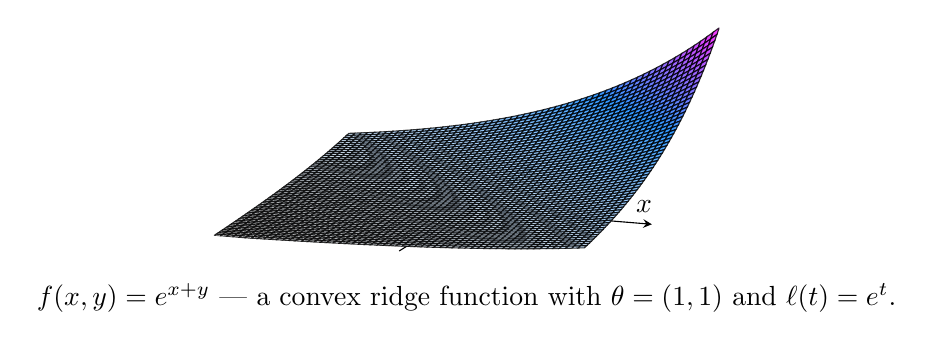
\begin{tikzpicture}
        \begin{axis}[
                view={20}{30},            % 3‑D view angle (azimuth, elevation)
                axis lines=center,
                width=8cm, height=5cm,   %  ⇐ make figure larger
                xlabel={$x$},
                % ylabel={$y$},
                % Hide tick labels (and optional tick marks) on x & y axes
                xtick=\empty, ytick=\empty,
                xticklabels={}, yticklabels={},
                % Hide the z‑axis completely
                z axis line style={opacity=0},
                zticklabels={}, ztick style={opacity=0},
                zlabel style={opacity=0},
                colormap/cool,             % pleasant blue‑purple gradient
                domain=-1:1,
                y domain=-1:1,
                samples=60, samples y=60,  % grid resolution (denser)
            ]
            % --- Function definition ---
            \addplot3[
                surf,
                draw=black,      % grid lines on the surface
                shader=flat,     % flat shading to emphasise mesh
                opacity=0.8,     % transparency so grid shows well
            ]{exp(x + y)};
        \end{axis}
        % Caption below the plot
        \node at (current bounding box.south) [below=8pt]{$f(x,y)=e^{x+y}$ — a convex ridge function with $\theta=(1,1)$ and $\ell(t)=e^{t}$.};
    \end{tikzpicture}
\end{frame}

%%%%%%%%%%%%%%%%%%%%%%%%%%%%%%%%%%%%%%%%%%%%%%%%%%%%
\begin{frame}{Lower bounds -- main results}
    \small
    The following lower bounds share the same construction.
    \begin{tcolorbox}[title=Lower Bound 4, colback=red!5, colframe=red!60!black]
        When $\cK = \ball_1 \subset \R^d$, there exists a prior $\xi$ on $\cF_{\pb\pl}$ such that
        \[
            \BReg_n(\text{TS}) \;\ge\; \tfrac12\min\!\bigl\{n,\;\frac{1}{4}e^{\Omega(d/32)}\bigr\}.
        \]
    \end{tcolorbox}
    \begin{tcolorbox}[title=Lower Bound 2, colback=red!5, colframe=red!60!black]
        Suppose that $\cK = \ball_1\subset \R^d$ and $d>256$.
        Then there exists a prior $\xi$ on $\cF_{\pb\pl}$ such that
        \[
            \Delta(\pi, \xi) \geq 2^{-19} \frac{d}{\log(d)} \sqrt{\cI(\pi, \xi)}\,,
        \]
        for all policies $\pi$ on $K$.
    \end{tcolorbox}
    \alert{Lower bound 2} shows that for general convex losses in $\R^d$ the \textbf{classical info-ratio machinery} cannot give regret better than the known \(\widetilde{O}(d^{1.5}\sqrt{n})\).
\end{frame}

%%%%%%%%%%%%%%%%%%%%%%%%%%%%%%%%%%%%%%%%%%%%%%%%%%%%
\begin{frame}{Lower bounds -- construction}
    \begin{columns}
        \begin{column}{0.7\textwidth}
            \begin{itemize}
                \item Idea:
                      \begin{enumerate}
                          \leftskip=-1em % Add right padding of 2em
                          \item All \textcolor{blue}{$f_\theta$}$\sim \xi$ are mostly equal to a fixed \textcolor{orange}{$f$} on $\ball_1$.
                          \item Uniform prior and no noise!
                      \end{enumerate}
                \item $\ts$ lower bound:
                      \begin{enumerate}
                          \leftskip=-1em % Add right padding of 2em
                          \item $\ts$ plays on the ``perimeter'' $\sphere_1$ where the minimizers are.
                          \item Suffers constant regret for $\exp(d)$ rounds.
                      \end{enumerate}
                \item IR lower bound:
                      \begin{enumerate}
                          \leftskip=-1em % Add right padding of 2em
                          \item Radial symmetry.
                          \item Optimize for $r$ in $\frac{\Delta(r)^2}{\cI(r)}$:
                                \begin{enumerate}
                                    \leftskip=-1em % Add right padding of 2em
                                    \item Closer to $0$, \textcolor{red}{very low inf.} with \textcolor{green!70!black}{good prob}.
                                    \item Closer to $\sphere_1$, \textcolor{green!70!black}{high inf.} with \textcolor{red}{very low prob.}
                                \end{enumerate}
                      \end{enumerate}
            \end{itemize}
        \end{column}
        \begin{column}{0.3\textwidth}
            \scalebox{0.4}{
                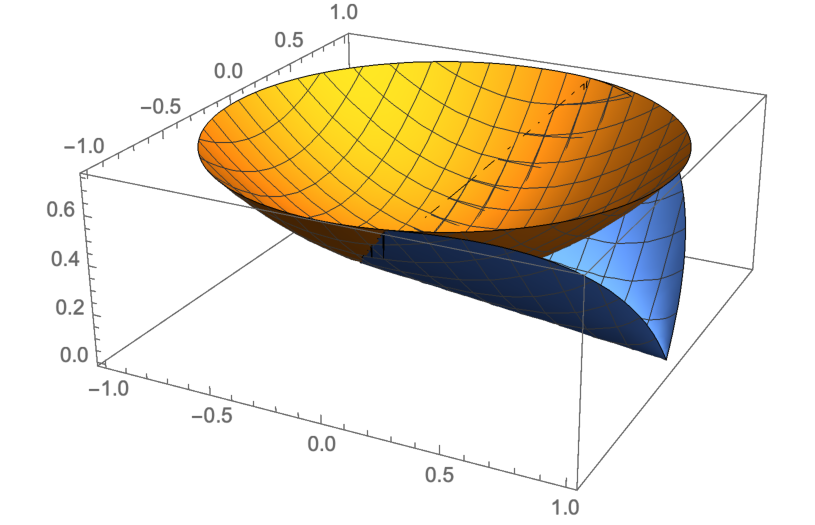
\includegraphics[width=10cm]{biconjugate}
            }
            \\
            \scalebox{0.4}{
                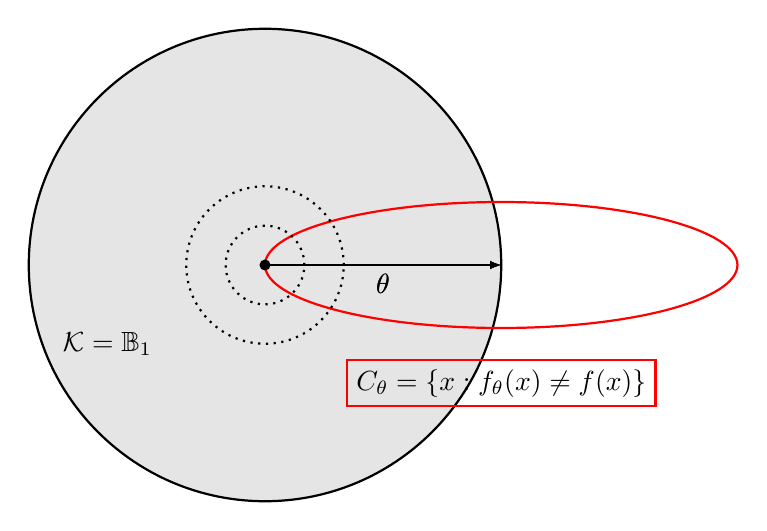
\begin{tikzpicture}
                    \draw[thick,fill=black!10!white] (0,0) circle (3);
                    \draw[thick,red] (3,0) ellipse (3 and 0.8);
                    \draw[fill=black,draw=none] (0,0) circle (2pt);
                    \draw (0,0) edge[-latex] node[below] {$\theta$} (3,0);
                    \draw (0,0) edge[-latex] node[below] {$\theta$} (3,0);
                    \node at (-2,-1) {$\cK = \ball_1$};
                    \node[draw=red,thick] at (3,-1.5) {$C_\theta = \{x : f_\theta(x) \neq f(x)\}$};
                    \draw[dotted,thick] (0,0) circle (1);
                    \draw[dotted,thick] (0,0) circle (0.5);
                \end{tikzpicture}
            }
        \end{column}
    \end{columns}
\end{frame}

%%%%%%%%%%%%%%%%%%%%%%%%%%%%%%%%%%%%%%%%%%%%%%%%%%%%
\begin{frame}{Paper in One Slide}
    \begin{itemize}
        \item \alert{Goal}: Understand how \textbf{Thompson Sampling (TS)} behaves in \textbf{bandit convex optimization (BCO)}.
        \item \textbf{Positive}:
              \begin{itemize}
                  \item $\BReg_n(\ts) = \widetilde{O}(\sqrt{n})$ in \emph{1-D} convex bandits.
                  \item $\BReg_n(\ts) = \widetilde{O}\!\bigl(d^{2.5}\sqrt{n}\bigr)$ for \emph{d-D monotone convex ridge} losses.
              \end{itemize}
        \item \textbf{Negative}:
              \begin{itemize}
                  \item TS can suffer \(\Omega(\exp(d))\) regret for general d-D convex losses.
                  \item Classical info-ratio tricks \(\Rightarrow\) no better than \(\widetilde{O}(d^{1.5}\sqrt{n})\) for general stochastic \& adversarial BCO.
              \end{itemize}
              % \item \textbf{Take-away}: TS is great in 1-D / structured convex settings, but not in full \(d\)-D.
    \end{itemize}
    \begin{center}
        Thanks!
    \end{center}
\end{frame}

%%%%%%%%%%%%%%%%%%%%%%%%%%%%%%%%%%%%%%%%%%%%%%%%%%%%
\end{document}